\documentclass[a4paper,12pt]{article} 

%%% Работа с русским языком
\usepackage{cmap}                           % поиск в PDF
\usepackage{mathtext} 			 	       % русские буквы в формулах
\usepackage[T2A]{fontenc}               % кодировка
\usepackage[utf8]{inputenc}              % кодировка исходного текста
\usepackage[english,russian]{babel}  % локализация и переносы
\usepackage{wrapfig}

\usepackage{amsmath,amsfonts,amssymb,amsthm,mathtools} % AMS
\usepackage{euscript}	 % Шрифт Евклид
\usepackage{mathrsfs} % Красивый матшрифт
\usepackage{graphicx}%Вставка картинок правильная
\usepackage{float}%"Плавающие" картинки
\usepackage{wrapfig}%Обтекание фигур (таблиц, картинок и прочего)
\title{Лабораторная работа 2.3.1 

Определение $\frac{C_P}{C_V}$ методом изобарического расширения}
\author{Кагарманов Радмир Б01-106}
\date{18 марта 2022 г.}

\begin{document}

\maketitle

\newpage

\paragraph{Цель работы:}определение $\frac{C_P}{C_V}$ для воздуха.
\paragraph{В работе используется:}стеклянный сосуд; U-образный жидкостный манометр; резиновая груша; газгольдер с воздухом; секундомер.
\paragraph{Экспериментальная установка \\}
Экспериментальная установка состоит из стеклянного сосуда А, снабжённого краном $\text{К}_1$ и U-образного жидкостного манометра, измеряющего избыточное давление газа в сосуде. Схема установки показана на рис. 1.

\begin{figure}[h]
\centering
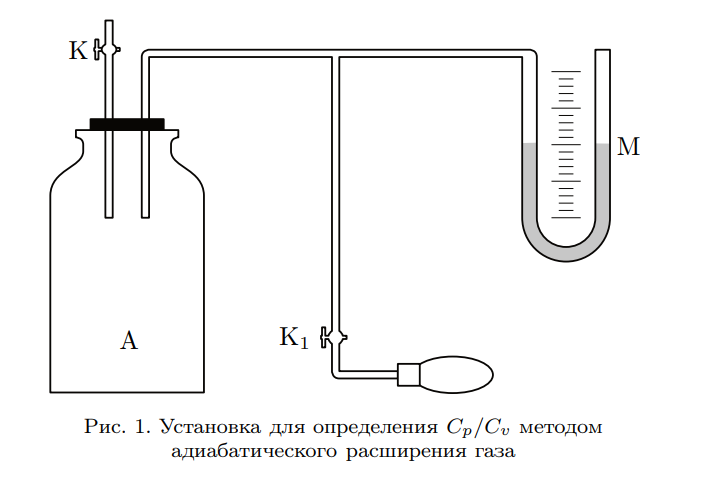
\includegraphics[width=0.7\linewidth]{установка.png}
\caption{Экспериментальная установка}
\label{fig:mpr}
\end{figure}
\\

С помощью резиновой груши, соединённой с трубкой краном $\text{K}_1$, в сосуде создаётся заданное избыточное $P_1$ воздуха. При этом газ оказывается перегретым.

Через некоторое время газ остынет до комнатной температуры $T_0$. Давление воздуха понизится до $P_0 + \Delta P_1$, где:

\begin{equation}
    \Delta P_1 = \rho g \Delta h_1
\end{equation}

Откроем кран $\text{K}$. За время $\Delta t$ порядка $0,5 с$ произойдёт адиабатическое расширение газа и его темература окажется ниже комнатной. Далее газ будет изобарически нагреваться. Зададим время $\tau$, в течение которого кран $\text{K}$ остаётся открытым, таким чтобы можно было пренебречь временем $\Delta t$.
После закрытия крана $\text{K}$ газ станет изохорически нагреваться до комнатной температуры, и давление газа возрастёт до $P_0 + \Delta P_2$, где:

\begin{equation}
    \Delta P_2 = \rho g \Delta h_2
\end{equation}

Будем считать воздух в газгольдере идеальным газом. Рассмотрим изобарическое расширение воздуха. Запишем уравнение теплового баланса для изменяющейся со временем массы $m=\frac{P_0 V_0}{RT}\mu$:

\begin{equation}
    c_p m dT = -\alpha (T-T_0)dt
\end{equation}

\begin{center}
    $c_p\frac{P_0 V_0}{RT}\mu = -\alpha (T-T_0)dt$  ~~или~~   $\frac{dT}{T(T-T_0)}=-\frac{\alpha dt}{c_p \frac{P_0 V_0}{R}\mu}$
\end{center}

Заметим, что~~  $\frac{1}{T(T-T_0)} = -\frac{1}{T_0}(\frac{1}{T}-\frac{1}{T-T_0})$, тогда ~~ $\frac{1}{T_0}(\frac{1}{T}-\frac{1}{T-T_0})=\frac{\alpha dt}{c_p m_0 T_0}$ \\
\par Выполним интегрирование:
\begin{center}
    $\int \limits^{T_2}_{T_1}(\frac{1}{T}-\frac{1}{T-T_0}) dT = \frac{\alpha}{c_p m_0}\int \limits^{\tau}_{0}dt$
\end{center}

Получим:

\begin{center}
    $\text{ln}(\frac{T_2}{T_1}) - \text{ln}(\frac{T_2 - T_0}{T_1 - T_0})=\frac{\alpha}{c_p m_0}\tau$ ~~или~~ $\text{ln}(\frac{T_2 \Delta T_1}{T_1 \Delta T_2})=\frac{\alpha}{c_p m_0}\tau$
\end{center}

Откуда:
\begin{equation}
    \frac{\Delta T_1}{T_1}=\frac{\Delta T_2}{T_2}\text{exp}(\frac{\alpha}{c_p m_0}\tau)
\end{equation}

Из соотношения для адиабатического расширения получим:
\begin{equation}
    \frac{\Delta T_1}{T_1}=\frac{(\gamma - 1)}{\gamma} \frac{\Delta P_1}{P_0}
\end{equation}

Из соотношения для изохорического нагрева:

\begin{equation}
    \frac{\Delta T_2}{T_2}=\frac{\Delta P_2}{P_0}
\end{equation}

Из (4), (5) и (6) получаем:
\begin{equation}
    \text{ln}(\frac{\Delta h_1}{\Delta h_2})=\text{ln}(\frac{\gamma}{\gamma - 1}) + \text{ln}(\frac{\alpha}{c_p m _0})\tau
\end{equation}
\newpage
\paragraph{Обработка результатов}
\subparagraph{1.} В таблице 1 представлены результаты измерений.
\begin{table}[h]
    \centering
    \begin{tabular}{|c|c|c|c|} \hline
        $\tau, с$ &  $\Delta h_1,см$ & $\Delta h_2, см$ & $\text{ln}\frac{\Delta h_1}{\Delta h_2}$\\ \hline
        5 &  21,6 & 4,3 & 1,614 \\ \hline
        10 & 20,4 & 3,1 & 1,884 \\ \hline
        15 & 17,6 & 2,3 & 2,035 \\ \hline
        20 & 18,7 & 1,8 & 2,341 \\ \hline
        25 & 20,7 & 1,6 & 2,560 \\ \hline
        30 & 21,6 & 1,3 & 2,810 \\ \hline
        35 & 19,5 & 1 & 2,970 \\ \hline
    \end{tabular}
    \caption{Измерения разницы уровней манометра}
    \label{tab:my_label}
\end{table}
\subparagraph{2.} Построим график зависимости $\text{ln}(\frac{\Delta h_1}{\Delta h_2})$ от $\tau$ и найдём $\text{ln}(\frac{\gamma}{\gamma - 1})$ с помощью МНК.
\subparagraph{3.} На рисунке 2 изображён этот график.
\begin{figure}[h]
\centering
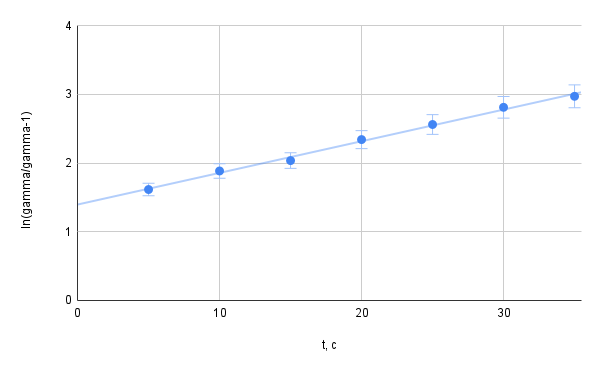
\includegraphics[width=0.7\linewidth]{nov.png}
\caption{График зависимости $\text{ln}(\frac{\Delta h_1}{\Delta h_2})$ от $\tau$}
\label{fig:mpr}
\end{figure} \\
$\text{ln}(\frac{\Delta h_1}{\Delta h_2}) = (0,0460 \pm 0,0014)\tau + (1,396 \pm 0,031)$
\subparagraph{4.} Найдём $\gamma$: 
\begin{center}
    $\frac{\gamma}{\gamma - 1}= e^{1,396}$\\
    $\gamma = 4,039\cdot \gamma - 4,039$\\
    $\gamma = 1,329$
\end{center}
\subparagraph{5.} Найдём погрешность $\gamma$: $\gamma = \frac{e^a}{e^a - 1}$ \\
$\varepsilon_\gamma = |\frac{e^a}{(e^a - 1)^2}\cdot \Delta a| \approx 1,4\%$\\
И добавим к этому инструментальную погрешность Для $\Delta h1$ инструментальная относительная погрешность порядка - $0,5\%$; для h2 - $5\%$; для гаммы, погрешность которой я нашёл из МНК, получается $1,4\%$; для времени инструментальная погрешность составляет - $1\%$. При сложении инструментальной и МНК погрешности как независимых получаем: $7,9\%$. \\
$\gamma = 1,33 \pm 0,11$
\paragraph{Вывод \\}
В ходе этой работы мы экспериментально получили отношение $\frac{c_\text{p}}{c_\text{v}}$ для воздуха $\gamma = 1,33\pm 0,11$, что совпадает с табличным значением $\gamma = 1,44$ в пределах погрешности. 

\end{document}
